\documentclass[12pt]{article}

\usepackage[margin=1.0in]{geometry}
\usepackage{tikz}
\usepackage{tabto}
\usetikzlibrary{automata,positioning}
\usepackage{enumitem}
\usepackage{amsmath}
\usepackage{amssymb}
\usetikzlibrary{automata,positioning}

\begin{document}

\title{CS4384 : Automata Theory\\Homework Assignment 1}
\author{Matthew McMillian\\mgm160130@utdallas.edu}
\maketitle


\begin{enumerate}
	
	\item Let $B$ $\subset$ $N_1$ (given) be a finite set of positive integers and define $\Sigma$ = $\{a, b\}$. \textit{Mathematically} define a DFA, $A$, that accepts a string $s \in \Sigma^*$ if and only if $\forall_{i \in B}$, the $i^{th}$ symbol of $s$ is $b$. \\
	
	We immediately define a this new DFA's $\Sigma$, $Q$, $Q_0$, and $F$ based off the criteria in the question. 
	\begin{itemize}
		\item[] $\Sigma$ = $\{a, b\}$, the alphabet of both sets.
		\item[] $Q$ = $[0, n]$ $\cap$ $\mathbb{N}_0$, where $n$ = max(B $\cup$ $\{0\}$). We define $n$ in such a that the maximum number of states that we need is the maximum number required in $B$ since we can loop back on the final $n$ state as an accepting state after $B$'s criteria is satisfied. We intersect with $\mathbb{N}_0$ to ensure our set of states are states numbered greater than 0.
		\item[] $Q_0$ = 0, our start state is defined to be state 0.
		\item[] $F$ = $\{0, n\}$, our set of accepting states. 0 is an accepting state since we must accept the empty set, and n is our final state that satisfies $B$'s requirements.
		\item[] The transition function can be broken down into 3 parts.
			\begin{itemize}
				\item We define an arbitrary set $S_1$ = $\{((q,b), q+1)$ $|$ $q, q+1 \in Q \}$. No matter what state we are in, it is OK to transition to the next state $q+1$ if our input is a $b$, since this will always satisfy $B$'s requirements.
				\item We define an arbitrary set $S_2$ = $\{((q,a), q+1)$ $|$ $q \in Q, q+1 \in Q - B \}$. We only want to transition to another state with an $a$ iff we are not transitioning to a state that $B$ requires as a $b$ transition.
				\item We define an arbitrary set $S_3$ = $\{((n,\sigma), n)$ $|$ $\sigma \in \Sigma\}$. This ensures that our case with the empty set, and our case that we finish looping through $B$ will accept anything after that input.
			\end{itemize}
		$\delta$ = $S_1$ $\cup$ $S_2$ $\cup$ $S_3$ = $\{((q,b), q+1)$ $|$ $q, q+1 \in Q \}$ $\cup$ $\{((q,a), q+1)$ $|$ $q \in Q, q+1 \in Q - B \}$ $\cup$ $\{((n,\sigma), n)$ $|$ $\sigma \in \Sigma\}$, which satisfies all of the cases in the DFA.
	\end{itemize}
	Thus, we define \fbox{A = ($Q$, $\Sigma$, $\delta$, $Q_0$, $F$)} respectively.
	\pagebreak
	
	\item Construct a DFA that accepts all binary strings divisible by 5.\\ \\
	For this problem, $\Sigma$ = $\{0, 1\}$, and $Q$ = $\{0 ,1, 2, 3, 4\}$. Our $\delta$, transition function, is defined as $Q$ $\times$ $\Sigma \rightarrow Q$, which means we should have $Q$ $\times$ $\Sigma$, $2 \times 5$, transitions in our diagram. Our $F$ = $\{0\}$. We can build a table modeling the relationships that our states should have until we have $Q$ $\times$ $\Sigma$ transitions. Then we can build our DFA out of the table's transitions.
	\begin{center}
	\begin{tabular}{c c c c}
	Number & Mod5 & Binary & State \\ \hline
	1 & 1 & 1 & 1 \\
	2 & 2 & 10 & 2 \\
	3 & 3 & 11 & 3 \\
	4 & 4 & 100 & 4 \\
	5 & 0 & 101 & 0 \\
	6 & 1 & 110 & 1 \\
	7 & 2 & 111 & 2 \\
	8 & 3 & 1000 & 3 \\
	9 & 4 & 1001 & 4 \\
	10 & 0 & 1010 & 5 \\
	\end{tabular}
	\end{center}
	
	Now that we have our table, we can begin to build our DFA from it's transitions. 
	\\ \\ \\  \\ 
\begin{tikzpicture}[shorten >=1pt,node distance=6cm,on grid,auto] 
   \node[state,initial, accepting] (q_0)   {$q_0$}; 
   \node[state] (q_1) [above right=of q_0] {$q_1$}; 
   \node[state] (q_2) [below right=of q_0] {$q_2$}; 
   \node[state](q_3) [below right=of q_1] {$q_3$};
   \node[state](q_4) [below right=of q_3] {$q_4$};
    \path[->] 
    (q_0) edge [loop above] node {0} ()
          edge  node {1} (q_1)
    (q_1) edge[bend left, above] node {1} (q_3)
          edge  node {0} (q_2)
    (q_2) edge  node [swap] {0} (q_4) 
          edge  node {1} (q_0)
    (q_3) edge[bend left, below] node {0}  (q_1) 
          edge  node {1} (q_2)
    (q_4) edge  node [swap] {0} (q_3) 
          edge [loop above] node {1} ();
\end{tikzpicture}
	\pagebreak
	
\item Construct an NFA for the language $L$ = $\{w $ $|$ $w$ contains the substring $aba\}$. \\

For this NFA, $\Sigma$ = $\{w $ $|$ $w$ is any character$ \}$, and $Q$ = $\{0 ,1, 2, 3\}$. The following NFA satisfies the language $L$. \\ \\ \\

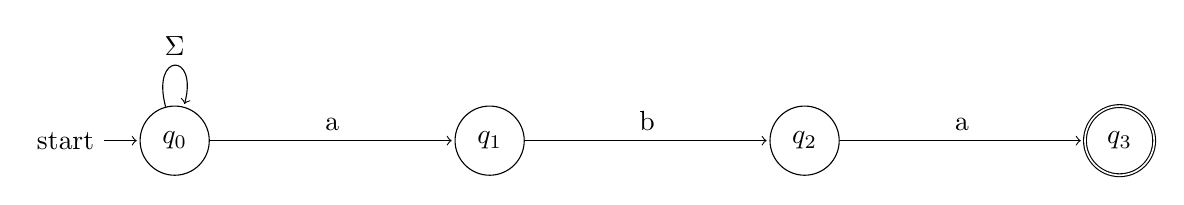
\begin{tikzpicture}[shorten >=1pt,node distance=4cm,on grid,auto] 
   \node[state,initial] (q_0)   {$q_0$}; 
   \node[state] (q_1) [right=of q_0] {$q_1$}; 
   \node[state] (q_2) [right=of q_1] {$q_2$}; 
   \node[state, accepting](q_3) [right=of q_2] {$q_3$};
    \path[->] 
    (q_0) edge  [loop above] node {$\Sigma$} ()
    	  edge node {a} (q_1)
    (q_1) edge node {b} (q_2)
    (q_2) edge  node {a} (q_3);
\end{tikzpicture}
	\pagebreak
	
	\item Convert the following NFAs to DFAs.
		\begin{itemize}
			\item[a.)] We construct 2 tables, 1 NFA table, and 1 DFA table. We get the values from the NFA table, and iteratively through filling out the DFA table.\\

\begin{table}[!htb]
    \caption{NFA to DFA}
    \begin{minipage}{.5\linewidth}
      \caption{NFA}
      \centering
        \begin{tabular}{c c c}
           q & a & b \\ \hline
	0 & 0,1 & 1 \\
	1 & - & 0  \\	
        \end{tabular}
    \end{minipage}%
    \begin{minipage}{.5\linewidth}
      \centering
        \caption{DFA}
        \begin{tabular}{c c c}
           q & a & b \\ \hline
	0 & 0,1 & 1 \\
	1 & - & 0  \\
	0,1 & 0,1 & 0,1 \\	
        \end{tabular}
    \end{minipage} 
\end{table}
	
	And we can then construct our DFA from the prior table. \\ \\ \\
		\begin{tikzpicture}[shorten >=1pt,node distance=8cm,on grid,auto] 
   \node[state,initial] (q_0)   {$q_0$}; 
   \node[state,accepting] (q_1) [above right=of q_0] {$q_1$}; 
   \node[state,accepting] (q_01) [below right=of q_1] {$q_{0,1}$}; 
    \path[->] 
    (q_0) edge node {a} (q_01)
    	  edge [bend left, above]  node {b} (q_1)
    (q_1) edge [bend left, below]  node {b} (q_0)
    (q_01) edge [loop above]  node {a,b} ();
          
\end{tikzpicture}\\
	\pagebreak
	\item[b.)] Similar to part a.), we construct 2 tables, 1 NFA table, and 1 DFA table. We get the values from the NFA table, and iteratively through filling out the DFA table.\\
	
	\begin{table}[!htb]
    \caption{NFA to DFA}
    \begin{minipage}{.5\linewidth}
      \caption{NFA}
      \centering
        \begin{tabular}{c c c}
           q & a & b \\ \hline
	0 & 0,1,2 & - \\
	1 & 0 & -  \\
	2 & 1 & 1,2  \\	
        \end{tabular}
    \end{minipage}%
    \begin{minipage}{.5\linewidth}
      \centering
        \caption{DFA}
        \begin{tabular}{c c c}
           q & a & b \\ \hline
	0 & 0,1,2 & - \\
	0,1,2 & 0,1,2 & 1,2  \\
	1,2 & 0,1 & 1,2 \\	
	0,1 & 0,1,2 & - \\
        \end{tabular}
    \end{minipage} 
\end{table}
	
	And we can then construct our DFA from the prior table. \\ \\ \\
		\begin{tikzpicture}[shorten >=1pt,node distance=7cm,on grid,auto] 
   \node[state,initial] (q_0)   {$q_0$}; 
    \node[state,accepting] (q_012) [above right=of q_0] {$q_{0,1,2}$};   
   \node[state,accepting] (q_01) [below right=of q_0] {$q_{0,1}$}; 
    \node[state,accepting] (q_12) [below right=of q_012] {$q_{1,2}$}; 
    \path[->] 
    (q_0) edge node {a} (q_012)    	 
    (q_12) edge  node {a} (q_01)
    		edge [loop right]  node {b} ()
    (q_01) edge  node {a} (q_012)        
    (q_012) edge [loop above] node {a} ()
   			edge  node {b} (q_12);
 
\end{tikzpicture}
	
\end{itemize}
\pagebreak

	\item Convert the following DFAs to REs. \\ \\
	We define Adren's Theorm below: \\
		\tabto{1cm} Let P, Q be regular expressions. If P $\neq$ $\emptyset$, then R = Q + RP = QP$^*$. 	
		\begin{itemize}
			\item[a.)] Regular Expression for DFA a., 
				\begin{itemize}
					\item[] $q_0$ = $aq_0 + bq_1 + \epsilon$
					\item[] $q_1$ = $aq_1 + bq_0$ = $bq_0a^*$ \tabto{9cm} (by Adren's Theorm)
					\item[] $q_0$ = $aq_0 + bbq_0a^* + \epsilon$
					\item[] $q_0$ = $q_0(a+ bba^*) + \epsilon$
					\item[] $q_0$ = $(a+ bba^*)^*$ \tabto{9cm}(by Adren's Theorm)
				\end{itemize}
				Thus our regular express for part a.) is \fbox{$(a+ bba^*)^*$}.
				
			\item[b.)] Regular Expression for DFA b., 
				\begin{itemize}
					\item[] $q_0$ = $aq_1 + bq_1 + \epsilon$
					\item[] $q_1$ = $aq_1 + bq_2$ 
					\item[] $q_2$ = $bq_1 + aq_0$ 
					\item[] $q_1$ = $aq_1 + b(bq_1 + aq_0)$ = $aq_1 + bbq_1 + aq_0$
					\item[] $q_1$ = $q_1(a + bb) + aq_0$ = $(a+bb)^*aq_0$ \tabto{9cm} (by Adren's Theorm)
					\item[] $q_0$ = $aa(a+bb)^*q_0 + ba(a+bb)^*q_0 + \epsilon$
					\item[] $q_0$ = $q_0(aa(a+bb)^* + ba(a+bb)^*) + \epsilon$
					\item[] $q_0$ = $(aa(a+bb)^* + ba(a+bb)^*)^*$ \tabto{9cm} (by Adren's Theorm)
				\end{itemize}
				Thus our regular express for part b.) is \fbox{$((aa + ba)(a+bb)^*)^*$}.
		\end{itemize}

\end{enumerate}


\end{document}
